% Created by tikzDevice version 0.10.1 on 2017-09-05 18:25:33
% !TEX encoding = UTF-8 Unicode
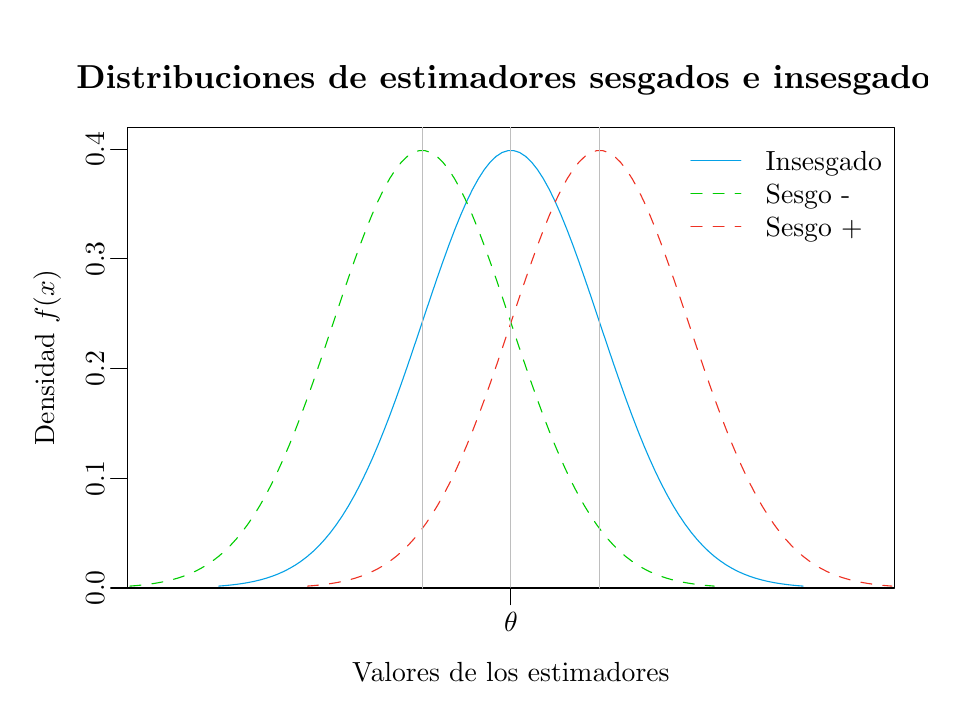
\begin{tikzpicture}[x=1pt,y=1pt]
\definecolor{fillColor}{RGB}{255,255,255}
\path[use as bounding box,fill=fillColor,fill opacity=0.00] (0,0) rectangle (325.21,238.49);
\begin{scope}
\path[clip] ( 36.00, 36.00) rectangle (313.21,202.49);
\definecolor{drawColor}{RGB}{5,161,230}

\path[draw=drawColor,line width= 0.4pt,line join=round,line cap=round] ( 69.02, 36.70) --
	( 71.15, 36.87) --
	( 73.28, 37.08) --
	( 75.42, 37.33) --
	( 77.55, 37.63) --
	( 79.68, 37.99) --
	( 81.81, 38.41) --
	( 83.95, 38.92) --
	( 86.08, 39.52) --
	( 88.21, 40.21) --
	( 90.35, 41.03) --
	( 92.48, 41.97) --
	( 94.61, 43.07) --
	( 96.75, 44.32) --
	( 98.88, 45.76) --
	(101.01, 47.39) --
	(103.15, 49.24) --
	(105.28, 51.32) --
	(107.41, 53.65) --
	(109.55, 56.24) --
	(111.68, 59.11) --
	(113.81, 62.27) --
	(115.95, 65.73) --
	(118.08, 69.50) --
	(120.21, 73.58) --
	(122.34, 77.97) --
	(124.48, 82.66) --
	(126.61, 87.66) --
	(128.74, 92.93) --
	(130.88, 98.47) --
	(133.01,104.25) --
	(135.14,110.22) --
	(137.28,116.37) --
	(139.41,122.64) --
	(141.54,128.99) --
	(143.68,135.37) --
	(145.81,141.71) --
	(147.94,147.96) --
	(150.08,154.06) --
	(152.21,159.94) --
	(154.34,165.55) --
	(156.48,170.80) --
	(158.61,175.66) --
	(160.74,180.05) --
	(162.88,183.92) --
	(165.01,187.22) --
	(167.14,189.92) --
	(169.27,191.97) --
	(171.41,193.36) --
	(173.54,194.06) --
	(175.67,194.06) --
	(177.81,193.36) --
	(179.94,191.97) --
	(182.07,189.92) --
	(184.21,187.22) --
	(186.34,183.92) --
	(188.47,180.05) --
	(190.61,175.66) --
	(192.74,170.80) --
	(194.87,165.55) --
	(197.01,159.94) --
	(199.14,154.06) --
	(201.27,147.96) --
	(203.41,141.71) --
	(205.54,135.37) --
	(207.67,128.99) --
	(209.80,122.64) --
	(211.94,116.37) --
	(214.07,110.22) --
	(216.20,104.25) --
	(218.34, 98.47) --
	(220.47, 92.93) --
	(222.60, 87.66) --
	(224.74, 82.66) --
	(226.87, 77.97) --
	(229.00, 73.58) --
	(231.14, 69.50) --
	(233.27, 65.73) --
	(235.40, 62.27) --
	(237.54, 59.11) --
	(239.67, 56.24) --
	(241.80, 53.65) --
	(243.94, 51.32) --
	(246.07, 49.24) --
	(248.20, 47.39) --
	(250.34, 45.76) --
	(252.47, 44.32) --
	(254.60, 43.07) --
	(256.73, 41.97) --
	(258.87, 41.03) --
	(261.00, 40.21) --
	(263.13, 39.52) --
	(265.27, 38.92) --
	(267.40, 38.41) --
	(269.53, 37.99) --
	(271.67, 37.63) --
	(273.80, 37.33) --
	(275.93, 37.08) --
	(278.07, 36.87) --
	(280.20, 36.70);
\end{scope}
\begin{scope}
\path[clip] (  0.00,  0.00) rectangle (325.21,238.49);
\definecolor{drawColor}{RGB}{0,0,0}

\path[draw=drawColor,line width= 0.4pt,line join=round,line cap=round] ( 36.00, 36.00) -- ( 36.00,194.56);

\path[draw=drawColor,line width= 0.4pt,line join=round,line cap=round] ( 36.00, 36.00) -- ( 30.00, 36.00);

\path[draw=drawColor,line width= 0.4pt,line join=round,line cap=round] ( 36.00, 75.64) -- ( 30.00, 75.64);

\path[draw=drawColor,line width= 0.4pt,line join=round,line cap=round] ( 36.00,115.28) -- ( 30.00,115.28);

\path[draw=drawColor,line width= 0.4pt,line join=round,line cap=round] ( 36.00,154.92) -- ( 30.00,154.92);

\path[draw=drawColor,line width= 0.4pt,line join=round,line cap=round] ( 36.00,194.56) -- ( 30.00,194.56);

\node[text=drawColor,rotate= 90.00,anchor=base,inner sep=0pt, outer sep=0pt, scale=  1.00] at ( 27.60, 36.00) {0.0};

\node[text=drawColor,rotate= 90.00,anchor=base,inner sep=0pt, outer sep=0pt, scale=  1.00] at ( 27.60, 75.64) {0.1};

\node[text=drawColor,rotate= 90.00,anchor=base,inner sep=0pt, outer sep=0pt, scale=  1.00] at ( 27.60,115.28) {0.2};

\node[text=drawColor,rotate= 90.00,anchor=base,inner sep=0pt, outer sep=0pt, scale=  1.00] at ( 27.60,154.92) {0.3};

\node[text=drawColor,rotate= 90.00,anchor=base,inner sep=0pt, outer sep=0pt, scale=  1.00] at ( 27.60,194.56) {0.4};

\path[draw=drawColor,line width= 0.4pt,line join=round,line cap=round] ( 36.00, 36.00) --
	(313.21, 36.00) --
	(313.21,202.49) --
	( 36.00,202.49) --
	( 36.00, 36.00);
\end{scope}
\begin{scope}
\path[clip] (  0.00,  0.00) rectangle (325.21,238.49);
\definecolor{drawColor}{RGB}{0,0,0}

\node[text=drawColor,anchor=base,inner sep=0pt, outer sep=0pt, scale=  1.20] at (174.61,216.35) {\bfseries Distribuciones de estimadores sesgados e insesgados};

\node[text=drawColor,anchor=base,inner sep=0pt, outer sep=0pt, scale=  1.00] at (174.61,  2.40) {Valores de los estimadores};

\node[text=drawColor,rotate= 90.00,anchor=base,inner sep=0pt, outer sep=0pt, scale=  1.00] at (  9.60,119.25) {Densidad $f(x)$};
\end{scope}
\begin{scope}
\path[clip] ( 36.00, 36.00) rectangle (313.21,202.49);
\definecolor{drawColor}{RGB}{0,205,0}

\path[draw=drawColor,line width= 0.4pt,dash pattern=on 4pt off 4pt ,line join=round,line cap=round] ( 36.93, 36.70) --
	( 39.06, 36.87) --
	( 41.20, 37.08) --
	( 43.33, 37.33) --
	( 45.46, 37.63) --
	( 47.60, 37.99) --
	( 49.73, 38.41) --
	( 51.86, 38.92) --
	( 54.00, 39.52) --
	( 56.13, 40.21) --
	( 58.26, 41.03) --
	( 60.40, 41.97) --
	( 62.53, 43.07) --
	( 64.66, 44.32) --
	( 66.79, 45.76) --
	( 68.93, 47.39) --
	( 71.06, 49.24) --
	( 73.19, 51.32) --
	( 75.33, 53.65) --
	( 77.46, 56.24) --
	( 79.59, 59.11) --
	( 81.73, 62.27) --
	( 83.86, 65.73) --
	( 85.99, 69.50) --
	( 88.13, 73.58) --
	( 90.26, 77.97) --
	( 92.39, 82.66) --
	( 94.53, 87.66) --
	( 96.66, 92.93) --
	( 98.79, 98.47) --
	(100.93,104.25) --
	(103.06,110.22) --
	(105.19,116.37) --
	(107.33,122.64) --
	(109.46,128.99) --
	(111.59,135.37) --
	(113.72,141.71) --
	(115.86,147.96) --
	(117.99,154.06) --
	(120.12,159.94) --
	(122.26,165.55) --
	(124.39,170.80) --
	(126.52,175.66) --
	(128.66,180.05) --
	(130.79,183.92) --
	(132.92,187.22) --
	(135.06,189.92) --
	(137.19,191.97) --
	(139.32,193.36) --
	(141.46,194.06) --
	(143.59,194.06) --
	(145.72,193.36) --
	(147.86,191.97) --
	(149.99,189.92) --
	(152.12,187.22) --
	(154.25,183.92) --
	(156.39,180.05) --
	(158.52,175.66) --
	(160.65,170.80) --
	(162.79,165.55) --
	(164.92,159.94) --
	(167.05,154.06) --
	(169.19,147.96) --
	(171.32,141.71) --
	(173.45,135.37) --
	(175.59,128.99) --
	(177.72,122.64) --
	(179.85,116.37) --
	(181.99,110.22) --
	(184.12,104.25) --
	(186.25, 98.47) --
	(188.39, 92.93) --
	(190.52, 87.66) --
	(192.65, 82.66) --
	(194.79, 77.97) --
	(196.92, 73.58) --
	(199.05, 69.50) --
	(201.18, 65.73) --
	(203.32, 62.27) --
	(205.45, 59.11) --
	(207.58, 56.24) --
	(209.72, 53.65) --
	(211.85, 51.32) --
	(213.98, 49.24) --
	(216.12, 47.39) --
	(218.25, 45.76) --
	(220.38, 44.32) --
	(222.52, 43.07) --
	(224.65, 41.97) --
	(226.78, 41.03) --
	(228.92, 40.21) --
	(231.05, 39.52) --
	(233.18, 38.92) --
	(235.32, 38.41) --
	(237.45, 37.99) --
	(239.58, 37.63) --
	(241.71, 37.33) --
	(243.85, 37.08) --
	(245.98, 36.87) --
	(248.11, 36.70);
\definecolor{drawColor}{RGB}{238,50,36}

\path[draw=drawColor,line width= 0.4pt,dash pattern=on 4pt off 4pt ,line join=round,line cap=round] (101.10, 36.70) --
	(103.23, 36.87) --
	(105.37, 37.08) --
	(107.50, 37.33) --
	(109.63, 37.63) --
	(111.77, 37.99) --
	(113.90, 38.41) --
	(116.03, 38.92) --
	(118.17, 39.52) --
	(120.30, 40.21) --
	(122.43, 41.03) --
	(124.57, 41.97) --
	(126.70, 43.07) --
	(128.83, 44.32) --
	(130.96, 45.76) --
	(133.10, 47.39) --
	(135.23, 49.24) --
	(137.36, 51.32) --
	(139.50, 53.65) --
	(141.63, 56.24) --
	(143.76, 59.11) --
	(145.90, 62.27) --
	(148.03, 65.73) --
	(150.16, 69.50) --
	(152.30, 73.58) --
	(154.43, 77.97) --
	(156.56, 82.66) --
	(158.70, 87.66) --
	(160.83, 92.93) --
	(162.96, 98.47) --
	(165.10,104.25) --
	(167.23,110.22) --
	(169.36,116.37) --
	(171.50,122.64) --
	(173.63,128.99) --
	(175.76,135.37) --
	(177.89,141.71) --
	(180.03,147.96) --
	(182.16,154.06) --
	(184.29,159.94) --
	(186.43,165.55) --
	(188.56,170.80) --
	(190.69,175.66) --
	(192.83,180.05) --
	(194.96,183.92) --
	(197.09,187.22) --
	(199.23,189.92) --
	(201.36,191.97) --
	(203.49,193.36) --
	(205.63,194.06) --
	(207.76,194.06) --
	(209.89,193.36) --
	(212.03,191.97) --
	(214.16,189.92) --
	(216.29,187.22) --
	(218.43,183.92) --
	(220.56,180.05) --
	(222.69,175.66) --
	(224.82,170.80) --
	(226.96,165.55) --
	(229.09,159.94) --
	(231.22,154.06) --
	(233.36,147.96) --
	(235.49,141.71) --
	(237.62,135.37) --
	(239.76,128.99) --
	(241.89,122.64) --
	(244.02,116.37) --
	(246.16,110.22) --
	(248.29,104.25) --
	(250.42, 98.47) --
	(252.56, 92.93) --
	(254.69, 87.66) --
	(256.82, 82.66) --
	(258.96, 77.97) --
	(261.09, 73.58) --
	(263.22, 69.50) --
	(265.35, 65.73) --
	(267.49, 62.27) --
	(269.62, 59.11) --
	(271.75, 56.24) --
	(273.89, 53.65) --
	(276.02, 51.32) --
	(278.15, 49.24) --
	(280.29, 47.39) --
	(282.42, 45.76) --
	(284.55, 44.32) --
	(286.69, 43.07) --
	(288.82, 41.97) --
	(290.95, 41.03) --
	(293.09, 40.21) --
	(295.22, 39.52) --
	(297.35, 38.92) --
	(299.49, 38.41) --
	(301.62, 37.99) --
	(303.75, 37.63) --
	(305.89, 37.33) --
	(308.02, 37.08) --
	(310.15, 36.87) --
	(312.28, 36.70);
\definecolor{drawColor}{RGB}{190,190,190}

\path[draw=drawColor,line width= 0.4pt,line join=round,line cap=round] (174.61, 36.00) -- (174.61,202.49);

\path[draw=drawColor,line width= 0.4pt,line join=round,line cap=round] (142.52, 36.00) -- (142.52,202.49);

\path[draw=drawColor,line width= 0.4pt,line join=round,line cap=round] (206.69, 36.00) -- (206.69,202.49);
\end{scope}
\begin{scope}
\path[clip] (  0.00,  0.00) rectangle (325.21,238.49);
\definecolor{drawColor}{RGB}{0,0,0}

\path[draw=drawColor,line width= 0.4pt,line join=round,line cap=round] (174.61, 36.00) -- (174.61, 36.00);

\path[draw=drawColor,line width= 0.4pt,line join=round,line cap=round] (174.61, 36.00) -- (174.61, 30.00);

\node[text=drawColor,anchor=base,inner sep=0pt, outer sep=0pt, scale=  1.00] at (174.61, 20.40) {$\theta$};
\end{scope}
\begin{scope}
\path[clip] ( 36.00, 36.00) rectangle (313.21,202.49);
\definecolor{drawColor}{RGB}{5,161,230}

\path[draw=drawColor,line width= 0.4pt,line join=round,line cap=round] (239.67,190.49) -- (257.67,190.49);
\definecolor{drawColor}{RGB}{0,205,0}

\path[draw=drawColor,line width= 0.4pt,dash pattern=on 4pt off 4pt ,line join=round,line cap=round] (239.67,178.49) -- (257.67,178.49);
\definecolor{drawColor}{RGB}{238,50,36}

\path[draw=drawColor,line width= 0.4pt,dash pattern=on 4pt off 4pt ,line join=round,line cap=round] (239.67,166.49) -- (257.67,166.49);
\definecolor{drawColor}{RGB}{0,0,0}

\node[text=drawColor,anchor=base west,inner sep=0pt, outer sep=0pt, scale=  1.00] at (266.67,187.05) {Insesgado};

\node[text=drawColor,anchor=base west,inner sep=0pt, outer sep=0pt, scale=  1.00] at (266.67,175.05) {Sesgo -};

\node[text=drawColor,anchor=base west,inner sep=0pt, outer sep=0pt, scale=  1.00] at (266.67,163.05) {Sesgo +};
\end{scope}
\end{tikzpicture}
